\section{Parameterbestimmung}

\begin{figure}[h!]
	\centering
	\begin{subfigure}{0.475\textwidth}
		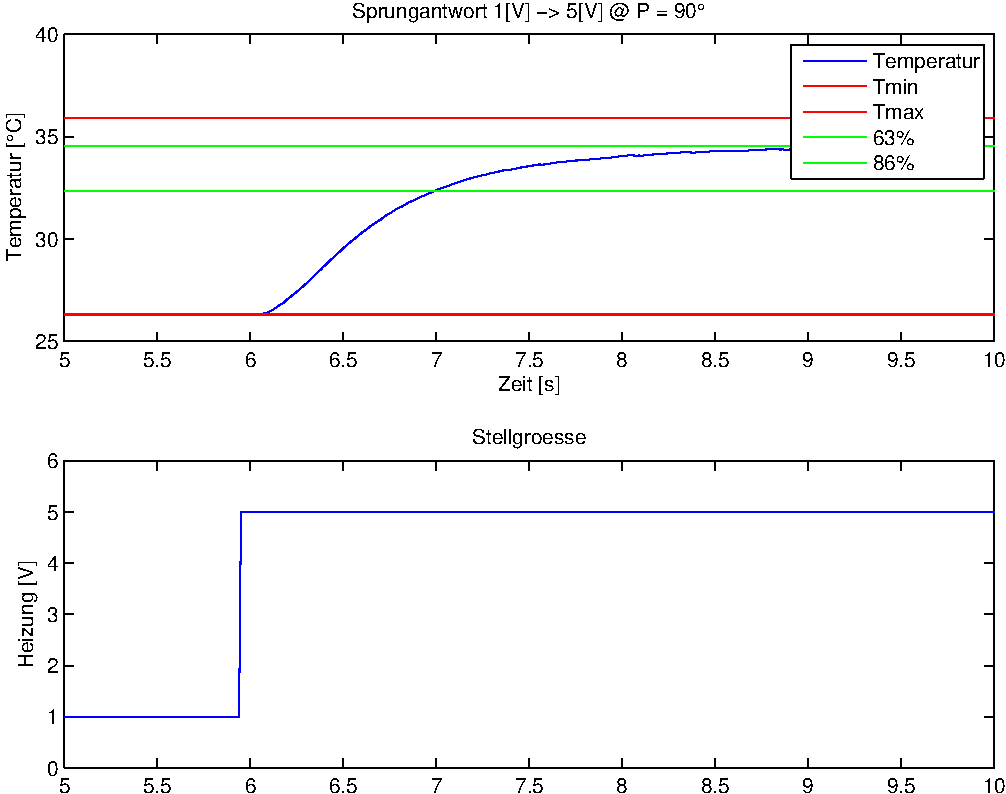
\includegraphics[width=1\textwidth]{04/step_plot_full_.pdf}
		\caption{Ventilstellung 90$^\circ$}
	\end{subfigure}
	\hfill{}
	\begin{subfigure}{0.475\textwidth}
		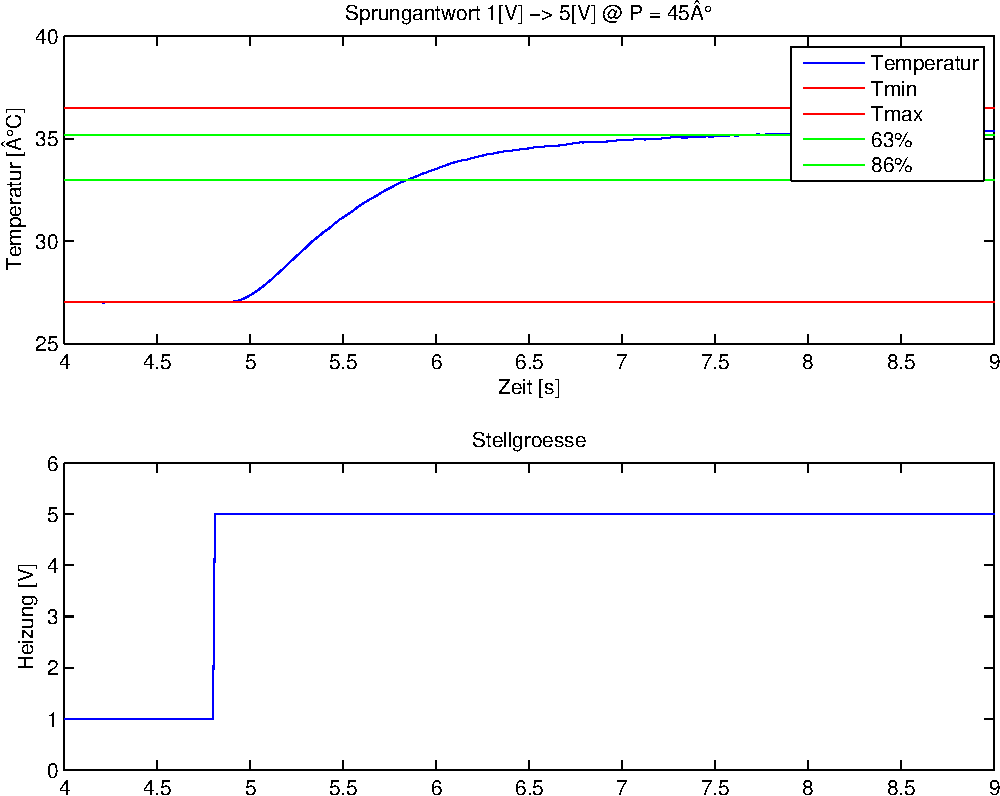
\includegraphics[width=1\textwidth]{04/step_plot_half_.pdf}
		\caption{Ventilstellung 45$^\circ$}
	\end{subfigure}
	\caption{Sprungantworten des Prozesses}
\end{figure}

Aus den Messdaten ergeben sich die folgenden Eckdaten
\begin{table}[h!]
	\centering
	\begin{tabular}{c c c c}
		Messwert
			& $\varphi = 90^\circ$
			& $\varphi = 45^\circ$
			& Einheit \\
		\hline
		$t_0$
			& 5.95
			& 4.81
			& $\si{\second}$ \\
		$\vartheta_{t_0}$
			& 26.31
			& 27.02
			& \si{\celsius} \\
		$\vartheta_{t_\infty}$
			& 35.9
			& 36.5
			& \si{\celsius} \\
		$t_{T_d}$
			& 6.12
			& 4.98
			& \si{\second} \\
	\end{tabular}
\end{table}

Mittels dieser Daten lassen sich die Eckwerte für die Parameterbestimmung
berechnen. Hierzu gehören die Werte, zu denen nach dem Zeit-Prozent-Verfahren
die Zeit zu ermitteln ist.
\[
	(\vartheta_\infty - \vartheta_0) \cdot n \% + \vartheta_0
	= \vartheta_{\tau_n}
\]

Mit diesem Verfahren ergeben sich die folgenden Werte für den Prozess
\begin{table}[h!]
	\centering
	\begin{tabular}{c c c c}
		Messwert
			& $\varphi = 90^\circ$
			& $\varphi = 45^\circ$
			& Einheit \\
		\hline
		$\vartheta_{\tau_1}$
			& 32.352
			& 32.992
			& $\si{\celsius}$ \\
		$\vartheta_{\tau_2}$
			& 34.557
			& 35.173
			& \si{\celsius} \\
		$t_{\tau_1}$
			& 6.99
			& 5.85
			& \si{\second} \\
		$t_{\tau_1}$
			& 10.02
			& 7.37
			& \si{\second} \\
	\end{tabular}
\end{table}

Mit diesen Werten lassen sich die die Parameter $K_g$ und $\tau$ des Prozesses
berechnen, welcher als PT$_1$T$_t$ zu modellieren ist. Dabei ergeben sich die
folgenden Werte
\begin{table}[h!]
	\centering
	\begin{tabular}{c c c c | l}
		Parameter
			& $\varphi = 90^\circ$
			& $\varphi = 45^\circ$
			& Einheit
			& Berechnung \\
		\hline
		$\tau_x$
			& 0.87
			& 0.87
			& $\si{\second}$
			& $(t_{\tau_1} - t_0)$ \\
		$\tau_y$
			& 3.03
			& 1.79
			& $\si{\second}$
			& $(t_{\tau_2} - t_{\tau_1})$ \\
		$\tau_z$
			& 1.95
			& 1.33
			& $\si{\second}$
			& $(\tau_2 - t_{T_d}) \cdot \frac{1}{2}$ \\
		$K_g$
			& 2.39
			& 2.37
			& $\si[per-mode=fraction]{\celsius\per\volt}$
			& $\frac{\Delta \vartheta}{\Delta u}$
	\end{tabular}
\end{table}

Diese Werte zeigen deutlich auf, dass es sich bei diesem Prozess um kein
reines PT$_1$T$_t$-Glied handeln kann. Bei einem idealen Glied dieser Art,
müssten sich für jeden Abschnitt die gleichen Zeitkonstanten ergeben.
Der anfängliche Anstieg ist jedoch bei beiden Arbeitspunkten des Prozesses
gleich ($\tau = 0.87\si{\second}$). Für die dynamischen Eigenschaften ist
dies die relevante Zeitkonstante. Ebenso ist auch das $K_g$ nahezu identisch.
Der Prozess verhält sich somit ähnlich für beide Arbeitspunkte
($\varphi = 90^\circ$, $\varphi = 45^\circ$).

\subsubsection{Fazit}
Je grösser die Luftzufuhr ist ($\varphi$ gross), desto schlechter kann die
durchströmende Luft aufgeheizt werden. Die Totzeit ist für alle beobachteten
Arbeitspunkte die selbe ($T_d =$ const.).


\subsection{Vergleich von Messdaten und Simulationsergebnissen}

\begin{figure}[h!]
    \centering
    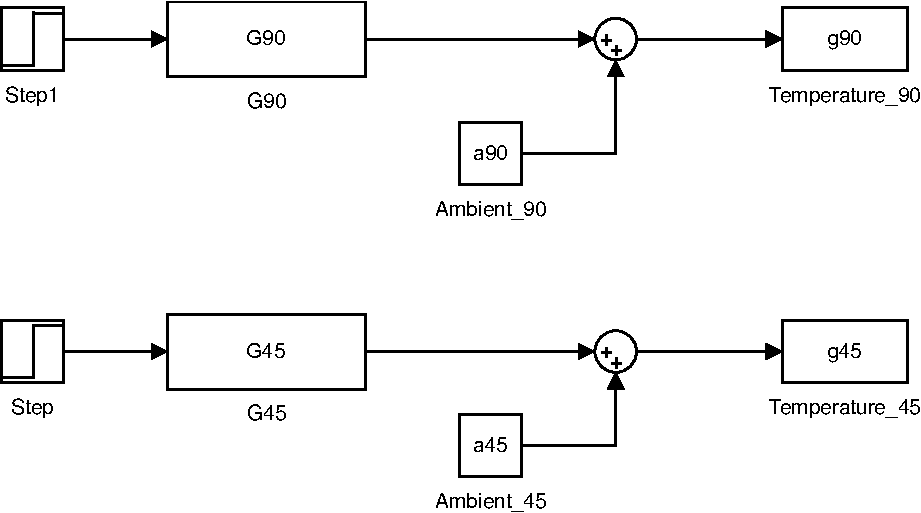
\includegraphics[scale=0.8]{04/model.pdf}
    \caption{Testmodell}
\end{figure}

\begin{figure}[h!]
    \begin{subfigure}{0.475\textwidth}
        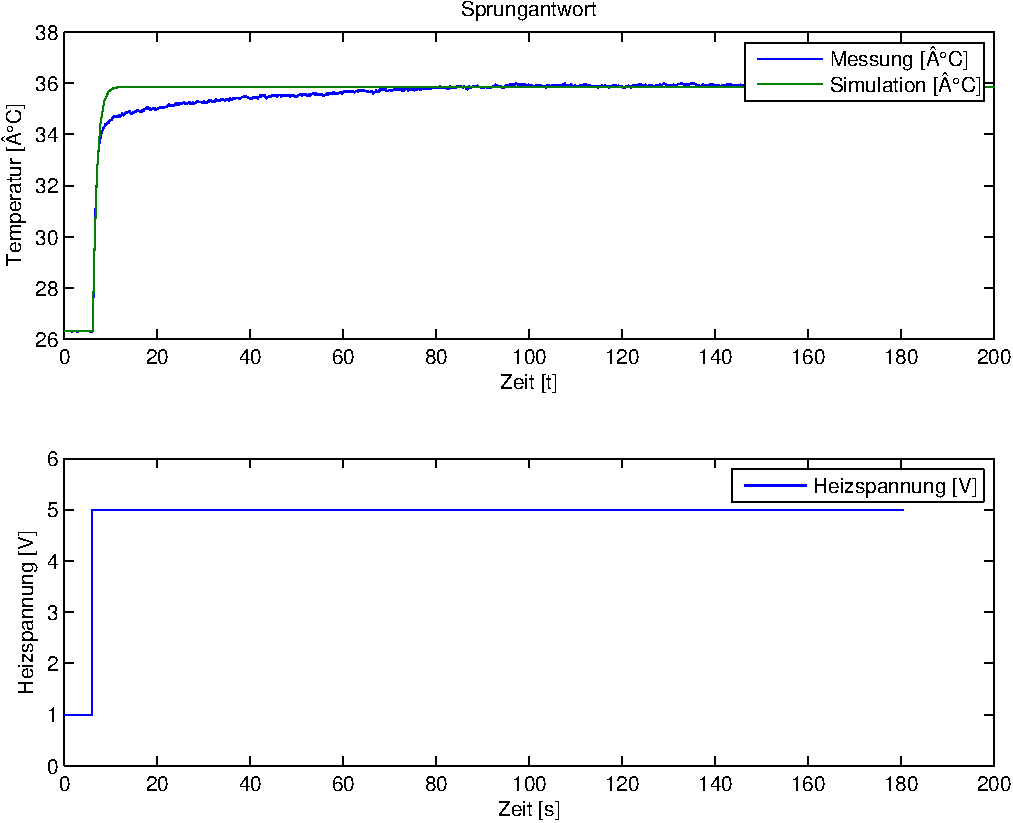
\includegraphics[width=1\textwidth]{04/step_mod_sim_90.pdf}
        \caption{Schrittantwort bei $\varphi = 90^\circ$}
    \end{subfigure}
    \hfill{}
    \begin{subfigure}{0.475\textwidth}
        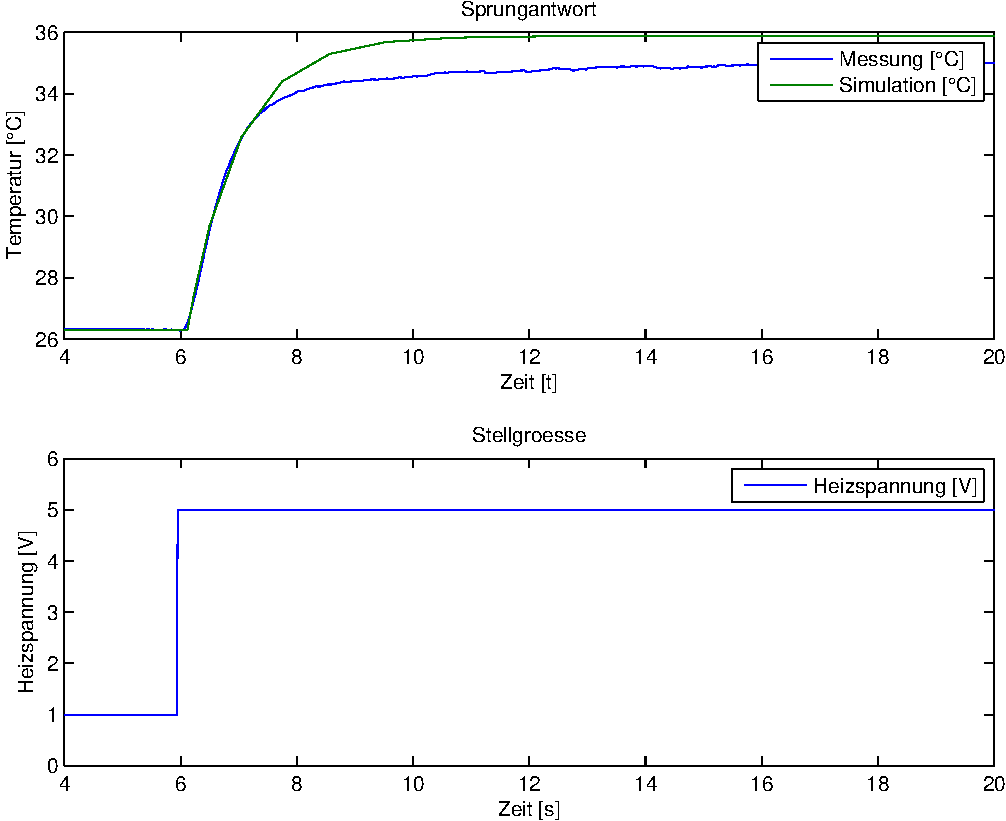
\includegraphics[width=1\textwidth]{04/step_mod_sim_90_scale.pdf}
        \caption{Schrittantwort skaliert auf Sprung bei $\varphi = 90^\circ$}
    \end{subfigure}
    \caption{Parameterkontrolle für $\varphi = 90^\circ$}
\end{figure}

\begin{figure}[h!]
    \begin{subfigure}{0.475\textwidth}
        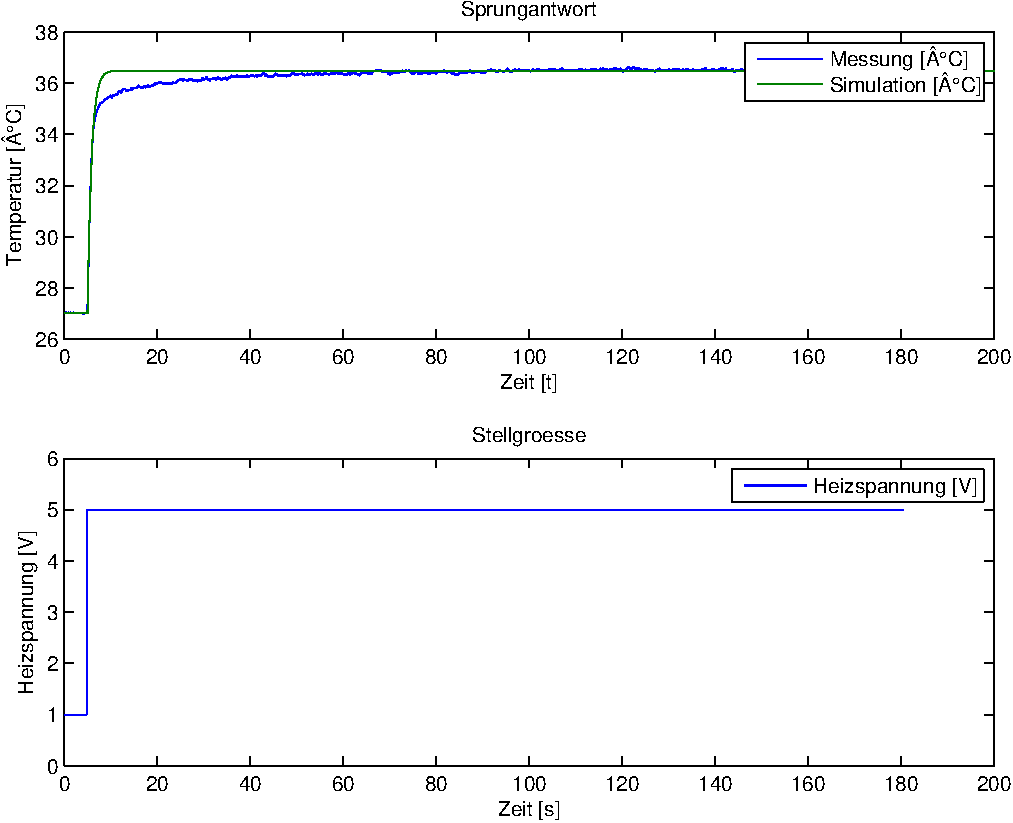
\includegraphics[width=1\textwidth]{04/step_mod_sim_45.pdf}
        \caption{Schrittantwort bei $\varphi = 45^\circ$}
    \end{subfigure}
    \hfill{}
    \begin{subfigure}{0.475\textwidth}
        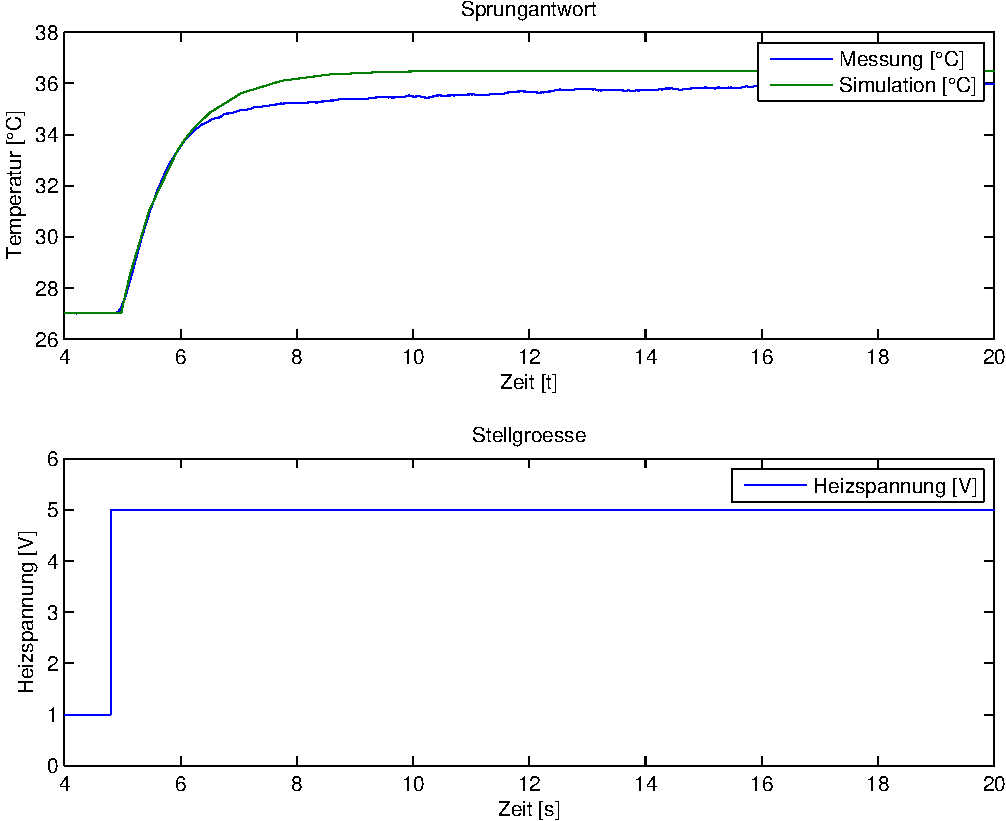
\includegraphics[width=1\textwidth]{04/step_mod_sim_45_scale.pdf}
        \caption{Schrittantwort skaliert auf Sprung bei $\varphi = 45^\circ$}
    \end{subfigure}
    \caption{Parameterkontrolle für $\varphi = 45^\circ$}
\end{figure}
